\documentclass[]{article}
\usepackage{lmodern}
\usepackage{amssymb,amsmath}
\usepackage{ifxetex,ifluatex}
\usepackage{fixltx2e} % provides \textsubscript
\ifnum 0\ifxetex 1\fi\ifluatex 1\fi=0 % if pdftex
  \usepackage[T1]{fontenc}
  \usepackage[utf8]{inputenc}
\else % if luatex or xelatex
  \ifxetex
    \usepackage{mathspec}
    \usepackage{xltxtra,xunicode}
  \else
    \usepackage{fontspec}
  \fi
  \defaultfontfeatures{Mapping=tex-text,Scale=MatchLowercase}
  \newcommand{\euro}{€}
\fi
% use upquote if available, for straight quotes in verbatim environments
\IfFileExists{upquote.sty}{\usepackage{upquote}}{}
% use microtype if available
\IfFileExists{microtype.sty}{%
\usepackage{microtype}
\UseMicrotypeSet[protrusion]{basicmath} % disable protrusion for tt fonts
}{}
\usepackage[margin=1in]{geometry}
\usepackage{color}
\usepackage{fancyvrb}
\newcommand{\VerbBar}{|}
\newcommand{\VERB}{\Verb[commandchars=\\\{\}]}
\DefineVerbatimEnvironment{Highlighting}{Verbatim}{commandchars=\\\{\}}
% Add ',fontsize=\small' for more characters per line
\usepackage{framed}
\definecolor{shadecolor}{RGB}{248,248,248}
\newenvironment{Shaded}{\begin{snugshade}}{\end{snugshade}}
\newcommand{\KeywordTok}[1]{\textcolor[rgb]{0.13,0.29,0.53}{\textbf{{#1}}}}
\newcommand{\DataTypeTok}[1]{\textcolor[rgb]{0.13,0.29,0.53}{{#1}}}
\newcommand{\DecValTok}[1]{\textcolor[rgb]{0.00,0.00,0.81}{{#1}}}
\newcommand{\BaseNTok}[1]{\textcolor[rgb]{0.00,0.00,0.81}{{#1}}}
\newcommand{\FloatTok}[1]{\textcolor[rgb]{0.00,0.00,0.81}{{#1}}}
\newcommand{\CharTok}[1]{\textcolor[rgb]{0.31,0.60,0.02}{{#1}}}
\newcommand{\StringTok}[1]{\textcolor[rgb]{0.31,0.60,0.02}{{#1}}}
\newcommand{\CommentTok}[1]{\textcolor[rgb]{0.56,0.35,0.01}{\textit{{#1}}}}
\newcommand{\OtherTok}[1]{\textcolor[rgb]{0.56,0.35,0.01}{{#1}}}
\newcommand{\AlertTok}[1]{\textcolor[rgb]{0.94,0.16,0.16}{{#1}}}
\newcommand{\FunctionTok}[1]{\textcolor[rgb]{0.00,0.00,0.00}{{#1}}}
\newcommand{\RegionMarkerTok}[1]{{#1}}
\newcommand{\ErrorTok}[1]{\textbf{{#1}}}
\newcommand{\NormalTok}[1]{{#1}}
\usepackage{longtable,booktabs}
\usepackage{graphicx}
\makeatletter
\def\maxwidth{\ifdim\Gin@nat@width>\linewidth\linewidth\else\Gin@nat@width\fi}
\def\maxheight{\ifdim\Gin@nat@height>\textheight\textheight\else\Gin@nat@height\fi}
\makeatother
% Scale images if necessary, so that they will not overflow the page
% margins by default, and it is still possible to overwrite the defaults
% using explicit options in \includegraphics[width, height, ...]{}
\setkeys{Gin}{width=\maxwidth,height=\maxheight,keepaspectratio}
\ifxetex
  \usepackage[setpagesize=false, % page size defined by xetex
              unicode=false, % unicode breaks when used with xetex
              xetex]{hyperref}
\else
  \usepackage[unicode=true]{hyperref}
\fi
\hypersetup{breaklinks=true,
            bookmarks=true,
            pdfauthor={Marco Torchiano},
            pdftitle={Analysis Procedure},
            colorlinks=true,
            citecolor=blue,
            urlcolor=blue,
            linkcolor=magenta,
            pdfborder={0 0 0}}
\urlstyle{same}  % don't use monospace font for urls
\setlength{\parindent}{0pt}
\setlength{\parskip}{6pt plus 2pt minus 1pt}
\setlength{\emergencystretch}{3em}  % prevent overfull lines
\setcounter{secnumdepth}{0}

%%% Use protect on footnotes to avoid problems with footnotes in titles
\let\rmarkdownfootnote\footnote%
\def\footnote{\protect\rmarkdownfootnote}

%%% Change title format to be more compact
\usepackage{titling}

% Create subtitle command for use in maketitle
\newcommand{\subtitle}[1]{
  \posttitle{
    \begin{center}\large#1\end{center}
    }
}

\setlength{\droptitle}{-2em}
  \title{Analysis Procedure}
  \pretitle{\vspace{\droptitle}\centering\huge}
  \posttitle{\par}
  \author{Marco Torchiano}
  \preauthor{\centering\large\emph}
  \postauthor{\par}
  \predate{\centering\large\emph}
  \postdate{\par}
  \date{19 November 2015}



\begin{document}

\maketitle


Computes the average power for the working tasks in a series of
measures.

The computation assumes the execution follows a well defined protocol to
mark tasks begin and end. A typical profile is:

\begin{verbatim}
       --------      --v-^v^--
       |      |      |       |
       |      |      |       |
 -------      --------       -....
  SLEEP: WAIT :SLEEP : WORK  :   
\end{verbatim}

\texttt{SLEEP} : is a period of sleep for a given (marker.length) time

\texttt{WAIT} : is a period of busy waiting for a given (marker.length)
time

\texttt{WORK} : is a period of actual work (the one we aim to measure
the energy consumption of)

\subsection{Load data}\label{load-data}

The analysis procedure can be applied on data containing Power samples.

Typically file containing current (\texttt{I}) values (expressed in
Ampere) is the starting point.

The power, given a \emph{constant} \texttt{voltage} in output from the
generator (5.03 V) -- can be computer using the basic relation

\[P=V \cdot I\]

\begin{Shaded}
\begin{Highlighting}[]
  \NormalTok{filepath =}\StringTok{ "data/syscall_mmap2.txt"}
  \CommentTok{#filepath = "data/syscall_futex.txt"}
  \CommentTok{#filepath = "data/syscall_gettimeofday.txt"}
  \CommentTok{#filepath = "data/syscall_mprotect.txt"}
  \NormalTok{voltage =}\StringTok{ }\FloatTok{5.03} \NormalTok{## Volt}

  \CommentTok{# read the file containing current values (in A)}
  \NormalTok{data =}\StringTok{ }\KeywordTok{read.delim2}\NormalTok{(filepath, }\DataTypeTok{header =} \OtherTok{FALSE}\NormalTok{, }\DataTypeTok{skip =} \DecValTok{7}\NormalTok{)}
  \KeywordTok{names}\NormalTok{(data)=}\StringTok{"I"}

\CommentTok{#  data = read.csv("~/Dropbox/PhDRifat/ENERGY ESEM 2015/Samples/Java/JavaBubble10000.csv")}
\CommentTok{#  names(data)[2]="I"}
\CommentTok{#  marker.length=1000}

  \CommentTok{# compute the power}
  \NormalTok{data$P <-}\StringTok{ }\KeywordTok{with}\NormalTok{(data, I*voltage )}
\end{Highlighting}
\end{Shaded}

\subsection{Input parameters}\label{input-parameters}

The algorithm takes the following input parameters:

\begin{Shaded}
\begin{Highlighting}[]
\NormalTok{adjust =}\StringTok{ }\FloatTok{1.5} \NormalTok{## density parameter}
\NormalTok{marker.length =}\StringTok{ }\DecValTok{5000}
\NormalTok{marker.tolerance=}\StringTok{ }\FloatTok{0.02}
\NormalTok{N =}\StringTok{ }\DecValTok{30} \CommentTok{# number of task markers}
\end{Highlighting}
\end{Shaded}

\subsection{Density analysis}\label{density-analysis}

Compute the distribution density of the instant power in order to
identify the typical working levels.

\begin{Shaded}
\begin{Highlighting}[]
  \NormalTok{## Distribution density of values}
  \NormalTok{dens <-}\StringTok{ }\KeywordTok{density}\NormalTok{(data$P,}\DataTypeTok{adjust=}\NormalTok{adjust)}
  \CommentTok{#dens <- density(data$P)}

  \NormalTok{## Find peaks in the distribution (the most common power levels)}
  \NormalTok{dens$peaks <-}\StringTok{ }\KeywordTok{which}\NormalTok{(}\KeywordTok{peaks}\NormalTok{(dens$y) &}\StringTok{ }\NormalTok{dens$y>}\KeywordTok{mean}\NormalTok{(dens$y))}

  \NormalTok{## Identify thresholds between peaks as the points of minimum density between peaks}
  \NormalTok{thresholds =}\StringTok{ }\NormalTok{dens$x[}\KeywordTok{apply}\NormalTok{(}\KeywordTok{cbind}\NormalTok{(}\KeywordTok{head}\NormalTok{(dens$peaks,-}\DecValTok{1}\NormalTok{),}\KeywordTok{tail}\NormalTok{(dens$peaks,-}\DecValTok{1}\NormalTok{)),}\DecValTok{1}\NormalTok{,function(x)\{}
    \NormalTok{ss =}\StringTok{ }\NormalTok{dens$y[x[}\DecValTok{1}\NormalTok{]:x[}\DecValTok{2}\NormalTok{]]}
    \NormalTok{x[}\DecValTok{1}\NormalTok{] +}\StringTok{ }\KeywordTok{which}\NormalTok{(ss ==}\StringTok{ }\KeywordTok{min}\NormalTok{(ss))}
  \NormalTok{\})]}

  \NormalTok{baseline =}\StringTok{ }\NormalTok{dens$x[dens$peaks[}\DecValTok{1}\NormalTok{]]}
\end{Highlighting}
\end{Shaded}

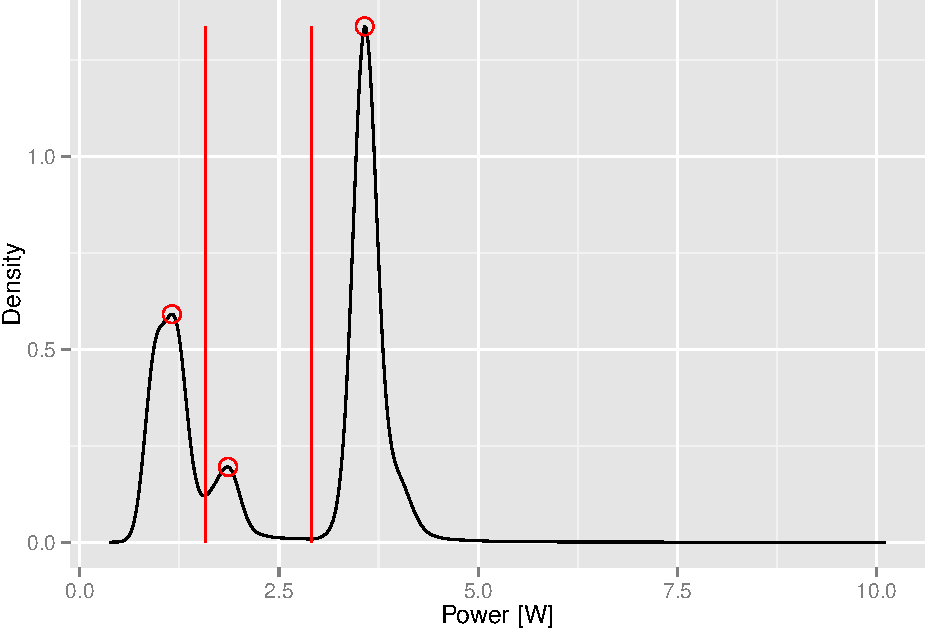
\includegraphics{AnalysisProcedure_files/figure-latex/density-1.pdf}

The baseline, representing the idle level of consumption correspond to
the first peak in the density plot: 1.1566972 W.

\subsection{Tagging}\label{tagging}

Each peak is assigned to a level, the the thresholds are used to
discriminate between consecutive levels. The data points are tagged with
the level name.

The tagging indetify runs of consecutive points having the same level.
The runs are then identified with a unique number.

To avoid manipulating the whole series of points, a summary table is
computed that reports:

\begin{itemize}
\itemsep1pt\parskip0pt\parsep0pt
\item
  tag
\item
  run ID
\item
  length
\item
  start position
\item
  end position
\end{itemize}

\begin{Shaded}
\begin{Highlighting}[]
  \NormalTok{## tag levels are those corresponding to peaks plus a special NOISE tag}
  \NormalTok{tag.levels <-}\StringTok{ }\KeywordTok{paste0}\NormalTok{(}\StringTok{"L"}\NormalTok{,}\KeywordTok{seq}\NormalTok{(dens$peaks))}
  \NormalTok{data$tag <-}\StringTok{ }\KeywordTok{factor}\NormalTok{(tag.levels[}\KeywordTok{findInterval}\NormalTok{(data$P,}\KeywordTok{c}\NormalTok{(}\DecValTok{0}\NormalTok{,thresholds))],}\KeywordTok{c}\NormalTok{(tag.levels,}\StringTok{"NOISE"}\NormalTok{))}

  \NormalTok{## assign unique id to runs}
  \NormalTok{data$runid <-}\StringTok{ }\KeywordTok{cumsum}\NormalTok{(}\KeywordTok{c}\NormalTok{(}\DecValTok{1}\NormalTok{,}\KeywordTok{abs}\NormalTok{(}\KeywordTok{diff}\NormalTok{(}\KeywordTok{as.numeric}\NormalTok{(data$tag))!=}\DecValTok{0}\NormalTok{) ) )}

  \NormalTok{## build run summary table}
  \NormalTok{id.tab =}\StringTok{ }\KeywordTok{subset}\NormalTok{(}\KeywordTok{melt}\NormalTok{(}\KeywordTok{with}\NormalTok{(data,}\KeywordTok{table}\NormalTok{(tag,runid)),}\DataTypeTok{id.vars=}\StringTok{"runid"}\NormalTok{,}\DataTypeTok{value.name=}\StringTok{"length"}\NormalTok{),length!=}\DecValTok{0}\NormalTok{)}
  \NormalTok{id.tab$start=}\KeywordTok{cumsum}\NormalTok{(}\KeywordTok{c}\NormalTok{(}\DecValTok{1}\NormalTok{,}\KeywordTok{head}\NormalTok{(id.tab$length,-}\DecValTok{1}\NormalTok{)))}
  \NormalTok{id.tab$end=}\KeywordTok{cumsum}\NormalTok{(id.tab$length)}
\end{Highlighting}
\end{Shaded}

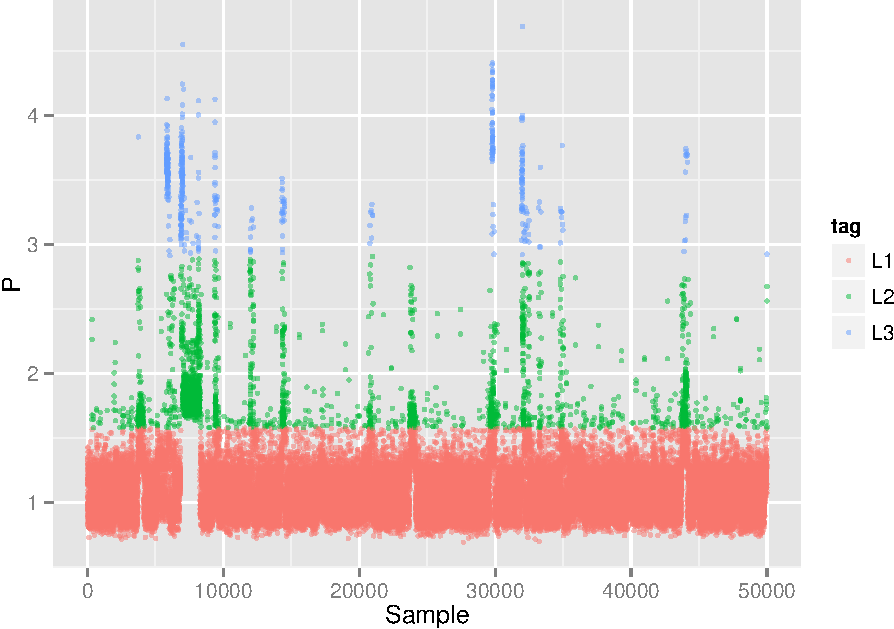
\includegraphics{AnalysisProcedure_files/figure-latex/tagged_data-1.pdf}
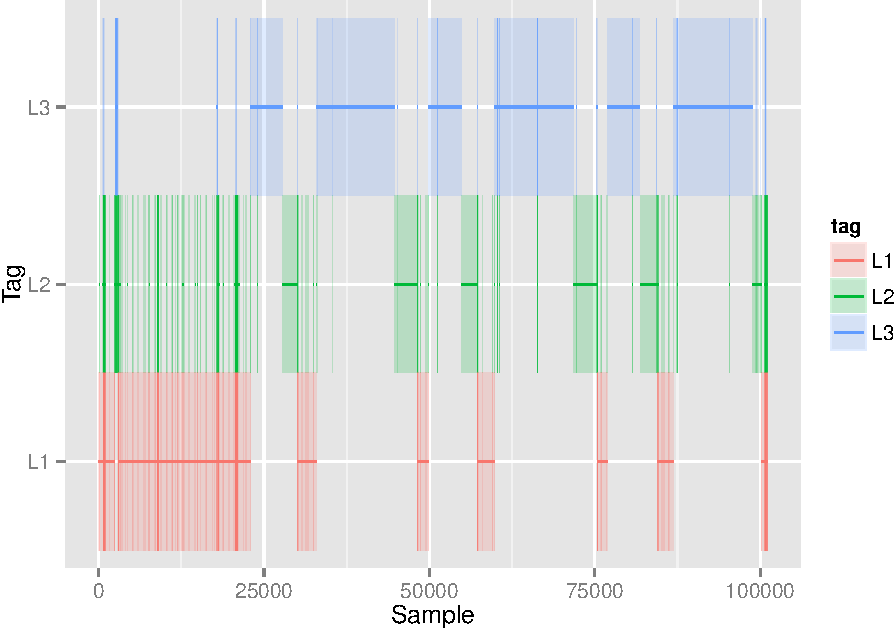
\includegraphics{AnalysisProcedure_files/figure-latex/tagged_data-2.pdf}

\subsection{Denoise}\label{denoise}

The collected measures are subject to noise (as any measure is).
Generally there are series of a few points that have a different value.

\begin{Shaded}
\begin{Highlighting}[]
  \NormalTok{dens =}\StringTok{ }\KeywordTok{density}\NormalTok{(id.tab$length)}
  \NormalTok{dens$peaks <-}\StringTok{ }\KeywordTok{which}\NormalTok{(}\KeywordTok{peaks}\NormalTok{(dens$y) &}\StringTok{ }\NormalTok{dens$y>}\KeywordTok{mean}\NormalTok{(dens$y))}

  \NormalTok{## Identify thresholds between peaks as the points of minimum density between peaks}
  \NormalTok{thresholds =}\StringTok{ }\NormalTok{dens$x[}\KeywordTok{apply}\NormalTok{(}\KeywordTok{cbind}\NormalTok{(}\KeywordTok{head}\NormalTok{(dens$peaks,-}\DecValTok{1}\NormalTok{),}\KeywordTok{tail}\NormalTok{(dens$peaks,-}\DecValTok{1}\NormalTok{)),}\DecValTok{1}\NormalTok{,function(x)\{}
    \NormalTok{ss =}\StringTok{ }\NormalTok{dens$y[x[}\DecValTok{1}\NormalTok{]:x[}\DecValTok{2}\NormalTok{]]}
    \NormalTok{x[}\DecValTok{1}\NormalTok{] +}\StringTok{ }\KeywordTok{which}\NormalTok{(ss ==}\StringTok{ }\KeywordTok{min}\NormalTok{(ss))}
  \NormalTok{\})]}
  \NormalTok{noise=thresholds[}\DecValTok{1}\NormalTok{]}
\end{Highlighting}
\end{Shaded}

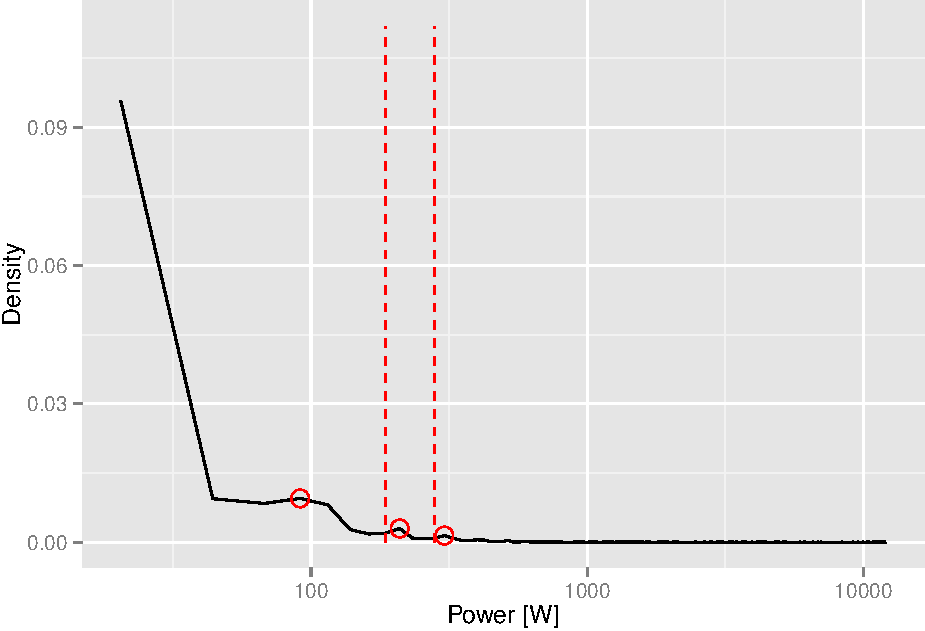
\includegraphics{AnalysisProcedure_files/figure-latex/noise_density-1.pdf}

A possible suggested threshold for noise is: 185.7085706

In most cases the nois is a small variation around the expected value.
Though, in some cases the noise is so large to cause a different tag to
be assigned.

We have, first, to identify the noise using a \texttt{noise} threshold
on the lenght of the runs.

\begin{Shaded}
\begin{Highlighting}[]
  \NormalTok{## identify noise runs by means of a run length threshold}
  \NormalTok{id.tab$tag[id.tab$length<noise] =}\StringTok{ "NOISE"}
\end{Highlighting}
\end{Shaded}

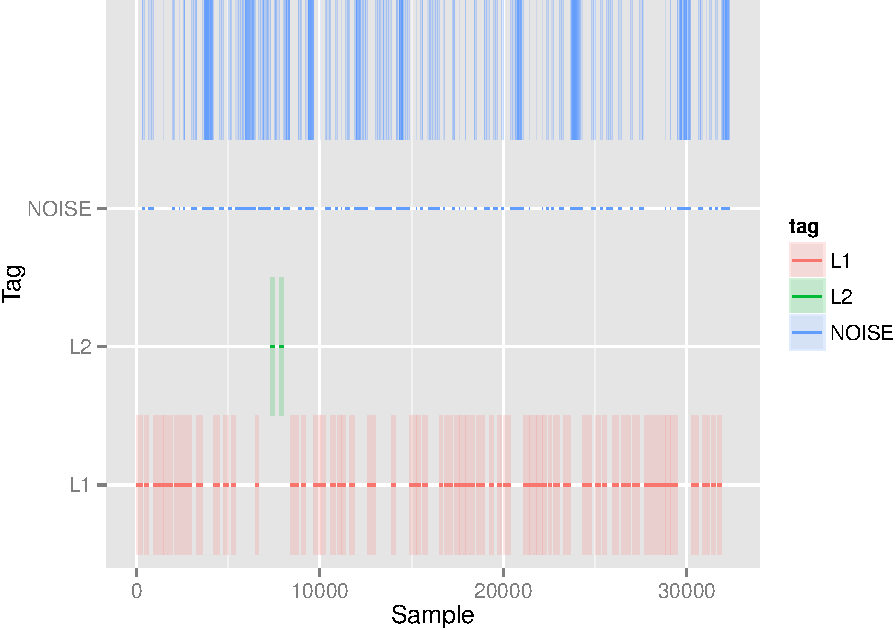
\includegraphics{AnalysisProcedure_files/figure-latex/runs_with_noise-1.pdf}

Then, we can remove the noise using some strategy:

\begin{itemize}
\itemsep1pt\parskip0pt\parsep0pt
\item
  merge noise run with the preceding run
\item
  merge the noise run with either the preceding or the following one,
  depending which is the largest.
\end{itemize}

\begin{Shaded}
\begin{Highlighting}[]
  \NormalTok{## Remove noise}
  \NormalTok{if(id.tab$tag[}\DecValTok{1}\NormalTok{]==}\StringTok{"NOISE"}\NormalTok{)\{}
    \NormalTok{id.tab$tag[}\DecValTok{1}\NormalTok{] =}\StringTok{ }\NormalTok{id.tab$tag[}\KeywordTok{min}\NormalTok{(id.tab$runid[id.tab$tag!=}\StringTok{"NOISE"}\NormalTok{])]}
  \NormalTok{\}}
  \NormalTok{id.noise =}\StringTok{ }\KeywordTok{which}\NormalTok{(id.tab$tag==}\StringTok{"NOISE"}\NormalTok{)}
  \NormalTok{while(}\KeywordTok{length}\NormalTok{(id.noise)>}\DecValTok{0}\NormalTok{)\{}
    \NormalTok{##  assign the noise run the same level as the  the preceding run}
    \NormalTok{id.tab$tag[id.noise] =}\StringTok{ }\NormalTok{id.tab$tag[id.noise}\DecValTok{-1}\NormalTok{]}
    \NormalTok{id.noise =}\StringTok{ }\KeywordTok{which}\NormalTok{(id.tab$tag==}\StringTok{"NOISE"}\NormalTok{)}
  \NormalTok{\}}
  \NormalTok{## id.tab = id.tab[order(id.tab$runid),] ### probably not useful}

  \NormalTok{## Merge consecutive runs havin the same tag}
  \NormalTok{## a) recompute the run id}
  \NormalTok{id.tab$runid =}\StringTok{ }\KeywordTok{cumsum}\NormalTok{(}\KeywordTok{c}\NormalTok{(}\DecValTok{1}\NormalTok{,}\KeywordTok{abs}\NormalTok{(}\KeywordTok{diff}\NormalTok{(}\KeywordTok{as.numeric}\NormalTok{(id.tab$tag))!=}\DecValTok{0}\NormalTok{) ) )}
  \NormalTok{## b) merge all the fragments with the same runid}
  \NormalTok{id.tab =}\StringTok{ }\KeywordTok{ddply}\NormalTok{(id.tab,.(runid,tag),summarize,}
                 \DataTypeTok{length =} \KeywordTok{sum}\NormalTok{(length),}
                 \DataTypeTok{start =} \KeywordTok{min}\NormalTok{(start),}
                 \DataTypeTok{end =} \KeywordTok{max}\NormalTok{(end)}
                 \NormalTok{)}
\end{Highlighting}
\end{Shaded}

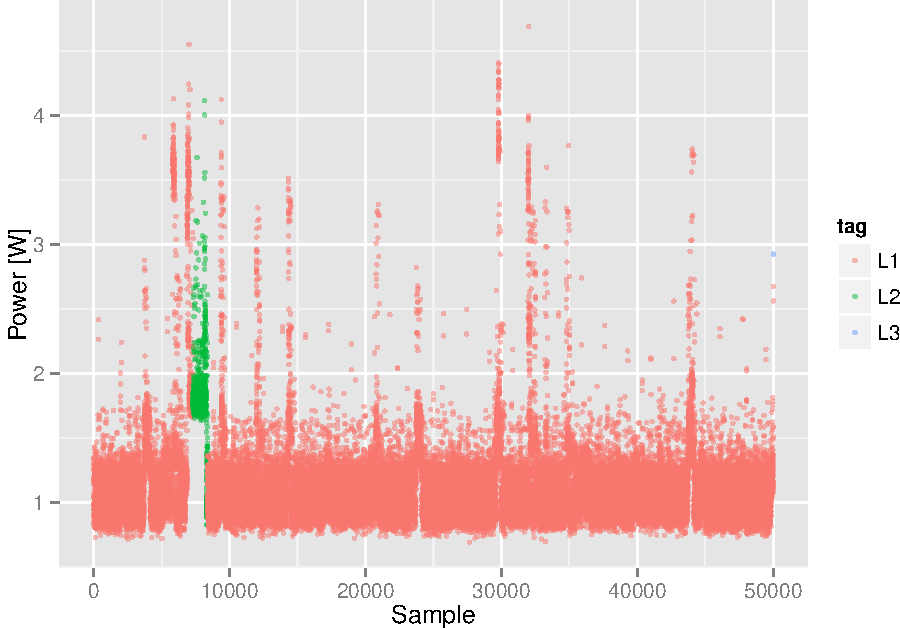
\includegraphics{AnalysisProcedure_files/figure-latex/denoised-1.pdf}
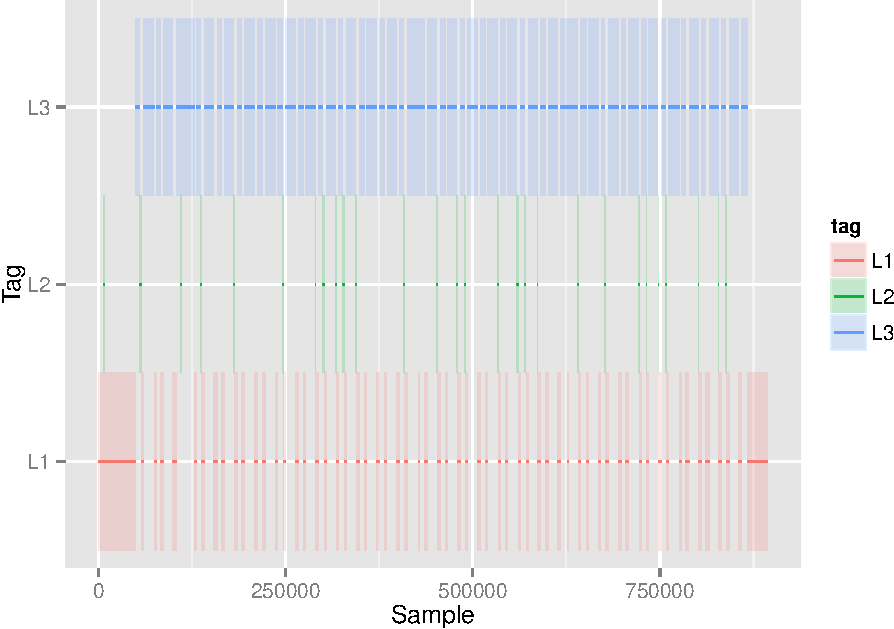
\includegraphics{AnalysisProcedure_files/figure-latex/denoised-2.pdf}

\begin{longtable}[c]{@{}rlrrr@{}}
\toprule
runid & tag & length & start & end\tabularnewline
\midrule
\endhead
1 & L1 & 7305 & 1 & 7305\tabularnewline
2 & L2 & 1070 & 7306 & 8375\tabularnewline
3 & L1 & 41624 & 8376 & 49999\tabularnewline
4 & L3 & 4910 & 50000 & 54909\tabularnewline
5 & L2 & 2355 & 54910 & 57264\tabularnewline
6 & L1 & 2725 & 57265 & 59989\tabularnewline
7 & L3 & 14171 & 59990 & 74160\tabularnewline
8 & L1 & 2872 & 74161 & 77032\tabularnewline
9 & L3 & 6448 & 77033 & 83480\tabularnewline
10 & L1 & 3559 & 83481 & 87039\tabularnewline
\bottomrule
\end{longtable}

\subsection{Identify task markers}\label{identify-task-markers}

Then we need to identify the marker that introduce the experiment.

We do not make any hypothesis as to the level at which markers are found
(it should be the highest one\ldots{})

The markers are (a subset of) the runs whose lenght is close to the
predefined marker length.

First we need to understand at which level (tag) are located the
markers.

For each distinct level/run:

\begin{itemize}
\item
  Count how many runs are in the expected range (the interval centered
  around \texttt{marker.length} with emiwidth
  \texttt{marker.tolerance}).
\item
  Compute the median period separating two consecutive runs
\item
  Compute the standard deviation of the period separating two
  consecutive runs
\item
  Select as marker level/tag the one with the number of potential
  markers, closer to the expected value (\texttt{N}) and with the
  smallest variability around of the period.
\end{itemize}

\begin{Shaded}
\begin{Highlighting}[]
  \NormalTok{l.min =}\StringTok{ }\NormalTok{marker.length*(}\DecValTok{1}\NormalTok{-marker.tolerance)}
  \NormalTok{l.max =}\StringTok{ }\NormalTok{marker.length*(}\DecValTok{1}\NormalTok{+marker.tolerance)}
  \NormalTok{markers =}\StringTok{ }\KeywordTok{subset}\NormalTok{(id.tab,length>=l.min &}\StringTok{ }\NormalTok{length<=l.max)}
  \NormalTok{mark.sum =}\StringTok{ }\KeywordTok{ddply}\NormalTok{(markers,.(tag),summarize,}
        \DataTypeTok{n=}\KeywordTok{length}\NormalTok{(tag),}
        \DataTypeTok{length =} \KeywordTok{median}\NormalTok{(length),}
        \DataTypeTok{t=} \KeywordTok{median}\NormalTok{(}\KeywordTok{diff}\NormalTok{(start)),}
\CommentTok{#        tv = sd(diff(start))}
\CommentTok{#        tv = 2*diff(quantile(diff(start),c(.25,.75)))}
        \DataTypeTok{tv =} \KeywordTok{median}\NormalTok{(}\KeywordTok{diff}\NormalTok{(start))*.}\DecValTok{02}
        \NormalTok{)}
  \NormalTok{mark.sum$score =}\StringTok{ }\KeywordTok{dim}\NormalTok{(mark.sum)[}\DecValTok{1}\NormalTok{]*(}\KeywordTok{rank}\NormalTok{(}\KeywordTok{abs}\NormalTok{(mark.sum$n-N))-}\DecValTok{1}\NormalTok{)+}\KeywordTok{rank}\NormalTok{(mark.sum$tv)-}\DecValTok{1}
  \NormalTok{marker =}\StringTok{ }\KeywordTok{subset}\NormalTok{(mark.sum,tag==}\KeywordTok{max}\NormalTok{(tag.levels))}
  \NormalTok{marker.tag =}\StringTok{ }\NormalTok{marker$tag}

  \KeywordTok{kable}\NormalTok{(mark.sum)}
\end{Highlighting}
\end{Shaded}

\begin{longtable}[c]{@{}lrrrrr@{}}
\toprule
tag & n & length & t & tv & score\tabularnewline
\midrule
\endhead
L3 & 6 & 5037.5 & 80680 & 1613.6 & 0\tabularnewline
\bottomrule
\end{longtable}

\begin{itemize}
\item
  the initial set of markers are the runs in the expected range
\item
  the we proceed with all the markers trying to find the next one either
  in the existing set of markers or in the runs with the market tag
\end{itemize}

\begin{Shaded}
\begin{Highlighting}[]
  \NormalTok{potential.markers =}\StringTok{ }\KeywordTok{subset}\NormalTok{(id.tab,tag==marker$tag)}

  \NormalTok{selected.markers =}\StringTok{ }\KeywordTok{c}\NormalTok{()}
  \NormalTok{initial.markers =}\StringTok{ }\KeywordTok{subset}\NormalTok{(markers,tag==marker$tag)}
  \KeywordTok{print}\NormalTok{(initial.markers$runid)}
\end{Highlighting}
\end{Shaded}

\begin{verbatim}
## [1]   4  13  17  51 130 145
\end{verbatim}

\begin{Shaded}
\begin{Highlighting}[]
  \NormalTok{generation =}\StringTok{ }\DecValTok{0}
  \NormalTok{while(!}\KeywordTok{is.null}\NormalTok{(initial.markers))\{}
    \NormalTok{generation <-}\StringTok{ }\NormalTok{generation +}\StringTok{ }\DecValTok{1}
    \NormalTok{if(generation >}\StringTok{ }\DecValTok{5}\NormalTok{) break}
    \NormalTok{new.markers=}\KeywordTok{c}\NormalTok{()}
    \NormalTok{for(id in initial.markers$runid)\{}
      \CommentTok{#cat(id,"\textbackslash{}n")}
      \NormalTok{current.marker =}\StringTok{ }\KeywordTok{subset}\NormalTok{(potential.markers,runid==id)}
      \NormalTok{t.expected =}\StringTok{ }\NormalTok{current.marker$start +}\StringTok{ }\NormalTok{marker$t}
      \NormalTok{t.lower =}\StringTok{ }\NormalTok{t.expected -}\StringTok{ }\NormalTok{marker$tv}
      \NormalTok{t.upper =}\StringTok{ }\NormalTok{t.expected +}\StringTok{ }\NormalTok{marker$tv}

      \NormalTok{successor =}\StringTok{ }\KeywordTok{subset}\NormalTok{(potential.markers,start>=t.lower &}\StringTok{ }\NormalTok{start<=t.upper &}\StringTok{ }\NormalTok{length>marker.length/}\DecValTok{2}\NormalTok{)}
      \NormalTok{if(}\KeywordTok{dim}\NormalTok{(successor)[}\DecValTok{1}\NormalTok{]>}\DecValTok{0}\NormalTok{)\{}
        \NormalTok{if(}\KeywordTok{dim}\NormalTok{(successor)[}\DecValTok{1}\NormalTok{]>}\DecValTok{1}\NormalTok{)\{}
          \NormalTok{successor <-}\StringTok{ }\KeywordTok{subset}\NormalTok{(successor,}\KeywordTok{abs}\NormalTok{(length-marker.length)==}\KeywordTok{min}\NormalTok{(}\KeywordTok{abs}\NormalTok{(length-marker.length)))}
          \CommentTok{#stop("No strategy to prioritize defined yet!!")}
        \NormalTok{\}}
        \NormalTok{if(!}\StringTok{ }\NormalTok{successor$runid%in%selected.markers$runid)\{}
          \NormalTok{new.markers <-}\StringTok{ }\KeywordTok{rbind}\NormalTok{(new.markers,successor)}
        \NormalTok{\}}
      \NormalTok{\}}

      \NormalTok{t.expected =}\StringTok{ }\NormalTok{current.marker$start -}\StringTok{ }\NormalTok{marker$t}
      \NormalTok{t.lower =}\StringTok{ }\NormalTok{t.expected -}\StringTok{ }\NormalTok{marker$tv}
      \NormalTok{t.upper =}\StringTok{ }\NormalTok{t.expected +}\StringTok{ }\NormalTok{marker$tv}
      \NormalTok{predecessor =}\StringTok{ }\KeywordTok{subset}\NormalTok{(potential.markers,start>=t.lower &}\StringTok{ }\NormalTok{start<=t.upper&}\StringTok{ }\NormalTok{length>marker.length/}\DecValTok{2}\NormalTok{)}
      \NormalTok{if(}\KeywordTok{dim}\NormalTok{(predecessor)[}\DecValTok{1}\NormalTok{]>}\DecValTok{0}\NormalTok{)\{}
        \NormalTok{if(}\KeywordTok{dim}\NormalTok{(predecessor)[}\DecValTok{1}\NormalTok{]>}\DecValTok{1}\NormalTok{)\{}
          \NormalTok{predecessor <-}\StringTok{ }\KeywordTok{subset}\NormalTok{(predecessor,}\KeywordTok{abs}\NormalTok{(length-marker.length)==}\KeywordTok{min}\NormalTok{(}\KeywordTok{abs}\NormalTok{(length-marker.length)))}
        \NormalTok{\}}
        \NormalTok{if(!}\StringTok{ }\NormalTok{predecessor$runid%in%selected.markers$runid)\{}
          \NormalTok{new.markers <-}\StringTok{ }\KeywordTok{rbind}\NormalTok{(new.markers,predecessor)}
        \NormalTok{\}}
      \NormalTok{\}}
    \NormalTok{\}}
    \NormalTok{new.markers =}\StringTok{ }\KeywordTok{unique}\NormalTok{(new.markers)}
    \NormalTok{initial.markers=new.markers}
    \NormalTok{if(!}\KeywordTok{is.null}\NormalTok{(new.markers))\{}
      \KeywordTok{print}\NormalTok{(new.markers$runid)}

      \NormalTok{new.markers$Gen =}\StringTok{ }\NormalTok{generation}
      \NormalTok{selected.markers=}\KeywordTok{rbind}\NormalTok{(selected.markers,new.markers)}
    \NormalTok{\}}
  \NormalTok{\}}
\end{Highlighting}
\end{Shaded}

\begin{verbatim}
## [1]  17  27  31   4  65  35 145 114 130
## [1]  40  13  45  80  51  22 101
## [1] 57 61 95  9 85
## [1]  70  75 110
## [1]  90 124
\end{verbatim}

\begin{Shaded}
\begin{Highlighting}[]
  \NormalTok{selected.markers <-}\StringTok{ }\KeywordTok{unique}\NormalTok{(selected.markers)}
  \NormalTok{selected.markers <-}\StringTok{ }\NormalTok{selected.markers[}\KeywordTok{order}\NormalTok{(selected.markers$runid),]}
\end{Highlighting}
\end{Shaded}

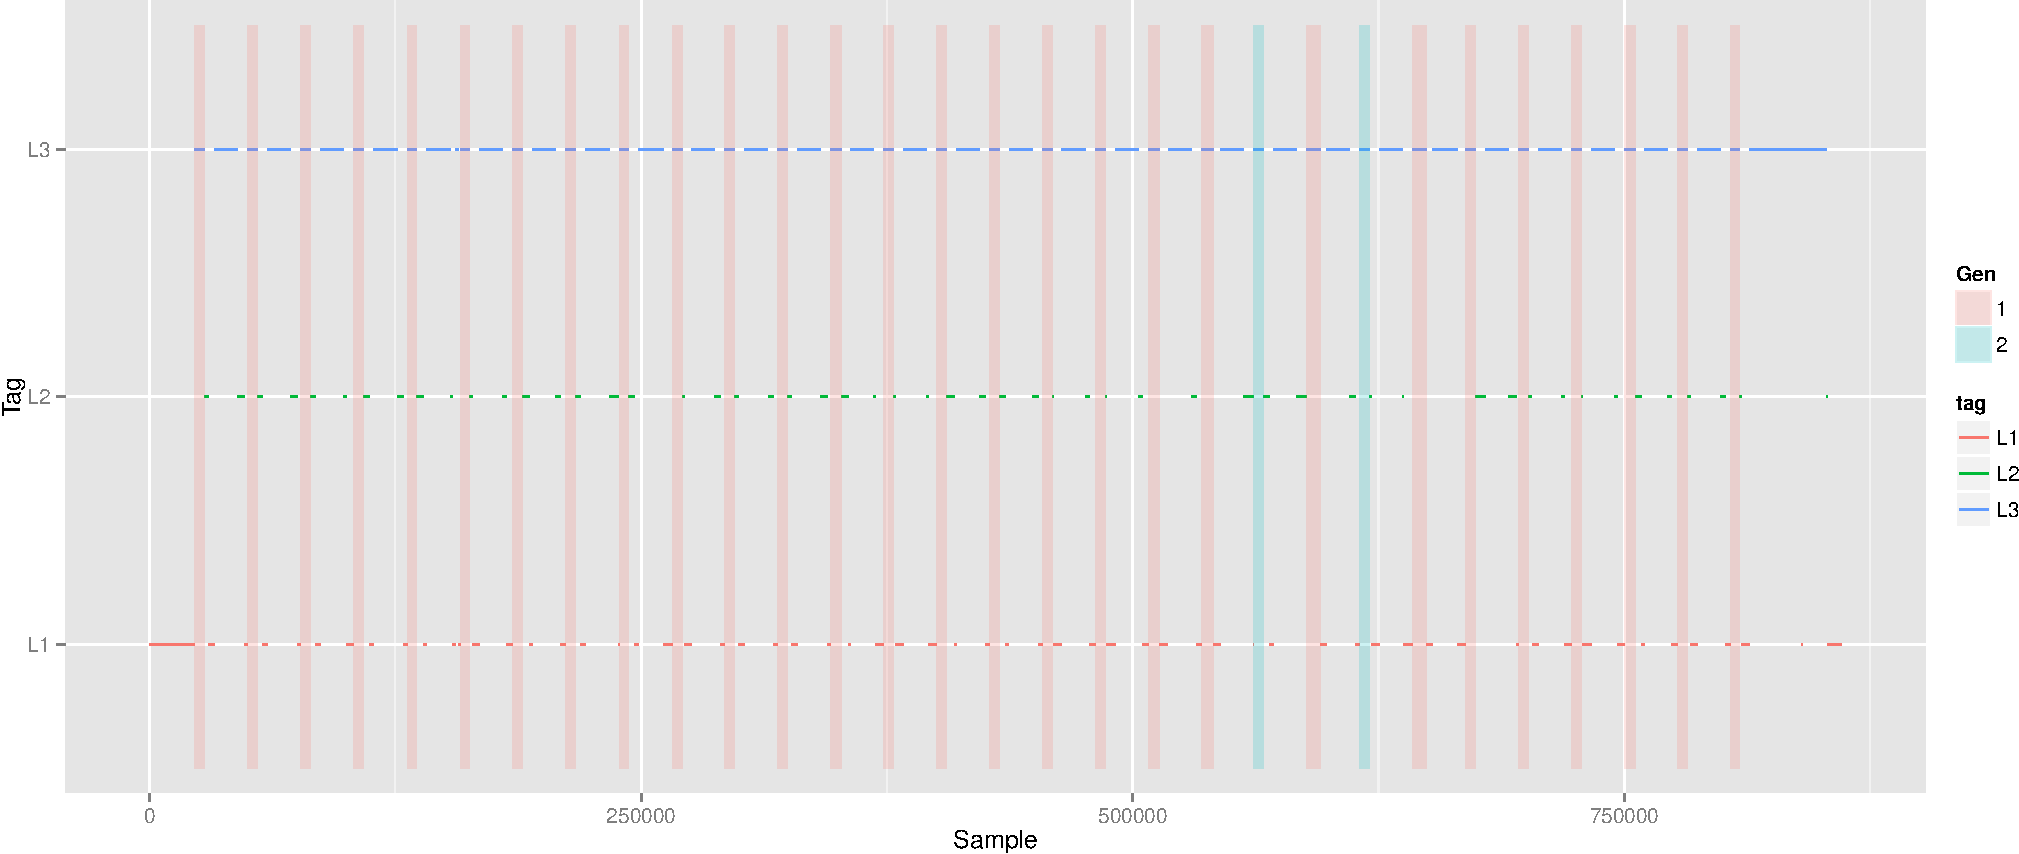
\includegraphics{AnalysisProcedure_files/figure-latex/runs_with_markers-1.pdf}

The procedure identified 26 markers. The average length of markers is
5873.2692308, median: 5735, sd: 757.292364.

\begin{longtable}[c]{@{}lrlrrrl@{}}
\toprule
& runid & tag & length & start & end & Gen\tabularnewline
\midrule
\endhead
4 & 4 & L3 & 4910 & 50000 & 54909 & 1\tabularnewline
9 & 9 & L3 & 6448 & 77033 & 83480 & 3\tabularnewline
13 & 13 & L3 & 5037 & 104139 & 109175 & 2\tabularnewline
17 & 17 & L3 & 5083 & 131211 & 136293 & 1\tabularnewline
22 & 22 & L3 & 5798 & 158363 & 164160 & 2\tabularnewline
27 & 27 & L3 & 5738 & 185470 & 191207 & 1\tabularnewline
31 & 31 & L3 & 6414 & 212542 & 218955 & 1\tabularnewline
35 & 35 & L3 & 5398 & 239762 & 245159 & 1\tabularnewline
40 & 40 & L3 & 6530 & 266903 & 273432 & 2\tabularnewline
45 & 45 & L3 & 5188 & 294112 & 299299 & 2\tabularnewline
51 & 51 & L3 & 4953 & 321150 & 326102 & 2\tabularnewline
57 & 57 & L3 & 7268 & 348290 & 355557 & 3\tabularnewline
61 & 61 & L3 & 6281 & 375390 & 381670 & 3\tabularnewline
65 & 65 & L3 & 5446 & 402502 & 407947 & 1\tabularnewline
70 & 70 & L3 & 6512 & 429432 & 435943 & 4\tabularnewline
75 & 75 & L3 & 7278 & 456313 & 463590 & 4\tabularnewline
80 & 80 & L3 & 5218 & 483249 & 488466 & 2\tabularnewline
85 & 85 & L3 & 6392 & 510141 & 516532 & 3\tabularnewline
90 & 90 & L3 & 6583 & 536983 & 543565 & 5\tabularnewline
95 & 95 & L3 & 5601 & 564060 & 569660 & 3\tabularnewline
101 & 101 & L3 & 5732 & 590792 & 596523 & 2\tabularnewline
110 & 110 & L3 & 7074 & 644492 & 651565 & 4\tabularnewline
114 & 114 & L3 & 5244 & 671302 & 676545 & 1\tabularnewline
124 & 124 & L3 & 6455 & 725003 & 731457 & 5\tabularnewline
130 & 130 & L3 & 5086 & 751932 & 757017 & 1\tabularnewline
145 & 145 & L3 & 5038 & 832612 & 837649 & 1\tabularnewline
\bottomrule
\end{longtable}

\subsection{Identify work}\label{identify-work}

For each marker, identify the beginning and end of the work run.

Possible options:

\begin{enumerate}
\def\labelenumi{\arabic{enumi}.}
\itemsep1pt\parskip0pt\parsep0pt
\item
  \textbf{End + T \emph{to} Start - T} (E2S): Skip a
  \texttt{marker.length} after marker \emph{end}: that's the beginning
  of a work; stop \texttt{marker.length} before the next marker
  \emph{start}
\end{enumerate}

\begin{Shaded}
\begin{Highlighting}[]
\NormalTok{work =}\StringTok{ }\KeywordTok{data.frame}\NormalTok{(}
      \DataTypeTok{start =} \KeywordTok{head}\NormalTok{(selected.markers,-}\DecValTok{1}\NormalTok{)$end+marker.length,}
      \DataTypeTok{end =} \KeywordTok{tail}\NormalTok{(selected.markers,-}\DecValTok{1}\NormalTok{)$start-marker.length}
      \NormalTok{)}
\NormalTok{work <-}\StringTok{ }\KeywordTok{within}\NormalTok{(work,}
       \NormalTok{length <-}\StringTok{ }\NormalTok{end-start}
       \NormalTok{)}
\KeywordTok{summary}\NormalTok{(work)}
\end{Highlighting}
\end{Shaded}

\begin{verbatim}
##      start             end             length     
##  Min.   : 59909   Min.   : 72033   Min.   : 9659  
##  1st Qu.:223955   1st Qu.:234762   1st Qu.:10495  
##  Median :386670   Median :397502   Median :11310  
##  Mean   :392128   Mean   :407527   Mean   :15399  
##  3rd Qu.:548565   3rd Qu.:559060   3rd Qu.:12036  
##  Max.   :762017   Max.   :827612   Max.   :65595
\end{verbatim}

\begin{enumerate}
\def\labelenumi{\arabic{enumi}.}
\setcounter{enumi}{1}
\itemsep1pt\parskip0pt\parsep0pt
\item
  \textbf{Start + 2 T \emph{to} Start - T} (S2S): Skip two
  \texttt{marker.length}s after marker \emph{end}: that's the beginning
  of a work; stop \texttt{marker.length} before the next marker
  \emph{start}
\end{enumerate}

\begin{Shaded}
\begin{Highlighting}[]
\NormalTok{work.run =}\StringTok{ }\KeywordTok{data.frame}\NormalTok{(}
      \DataTypeTok{start =} \KeywordTok{head}\NormalTok{(selected.markers,-}\DecValTok{1}\NormalTok{)$start}\DecValTok{+2}\NormalTok{*marker.length,}
      \DataTypeTok{end =} \KeywordTok{tail}\NormalTok{(selected.markers,-}\DecValTok{1}\NormalTok{)$start-marker.length}
      \NormalTok{)}
\NormalTok{work.run <-}\StringTok{ }\KeywordTok{within}\NormalTok{(work.run,}
       \NormalTok{length <-}\StringTok{ }\NormalTok{end-start}\DecValTok{+1}
       \NormalTok{)}
\KeywordTok{summary}\NormalTok{(work.run)}
\end{Highlighting}
\end{Shaded}

\begin{verbatim}
##      start             end             length     
##  Min.   : 60000   Min.   : 72033   Min.   :11733  
##  1st Qu.:222542   1st Qu.:234762   1st Qu.:11931  
##  Median :385390   Median :397502   Median :12078  
##  Mean   :391223   Mean   :407527   Mean   :16305  
##  3rd Qu.:546983   3rd Qu.:559060   3rd Qu.:12142  
##  Max.   :761932   Max.   :827612   Max.   :65681
\end{verbatim}

The second approach consistently gives better and more consistent
results.

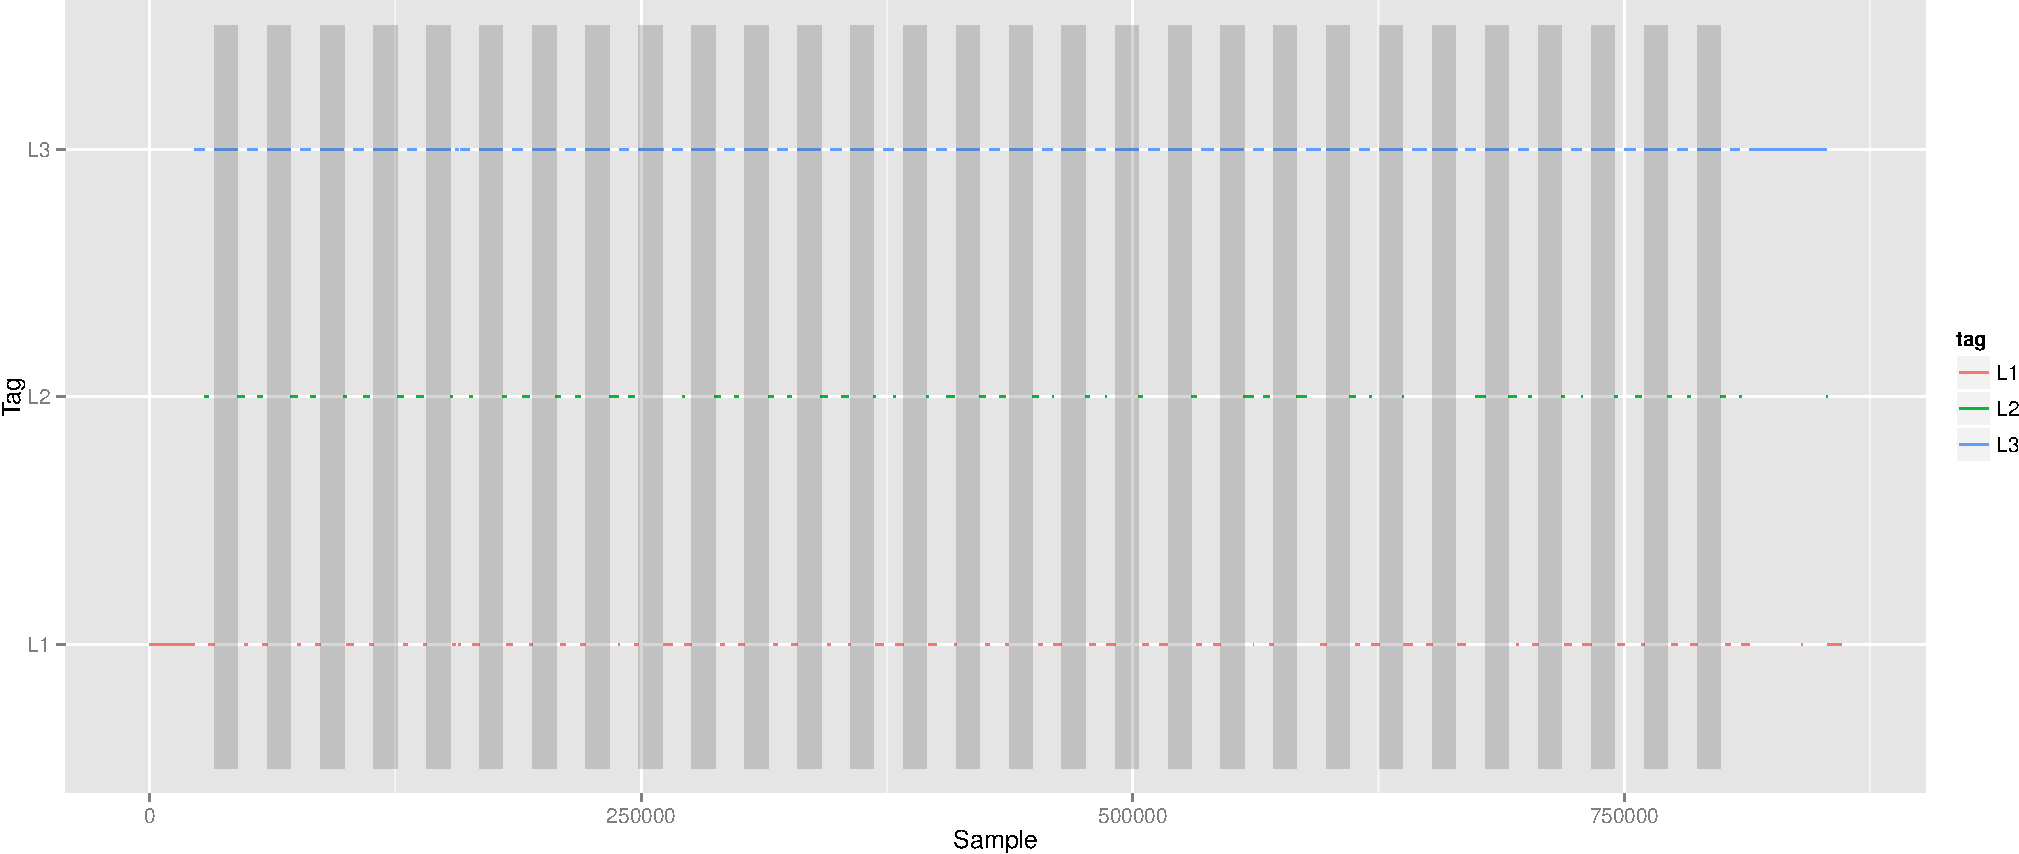
\includegraphics{AnalysisProcedure_files/figure-latex/work_runs_with_markers-1.pdf}

\subsection{Extract work data}\label{extract-work-data}

\begin{Shaded}
\begin{Highlighting}[]
\NormalTok{work.run$P <-}\StringTok{ }\KeywordTok{apply}\NormalTok{(work.run,}\DecValTok{1}\NormalTok{,function(x)}
                      \KeywordTok{mean}\NormalTok{(data[x[}\StringTok{"start"}\NormalTok{]:x[}\StringTok{"end"}\NormalTok{],]$P)-baseline)}
\end{Highlighting}
\end{Shaded}

\begin{Shaded}
\begin{Highlighting}[]
\NormalTok{p <-}\StringTok{ }\KeywordTok{ggplot}\NormalTok{(}\DataTypeTok{data=}\NormalTok{work.run,}\KeywordTok{aes}\NormalTok{(}\DataTypeTok{x=}\StringTok{''}\NormalTok{,}\DataTypeTok{y=}\NormalTok{P))+}\KeywordTok{geom_boxplot}\NormalTok{()}
\NormalTok{p <-}\StringTok{ }\NormalTok{p+}\KeywordTok{geom_segment}\NormalTok{(}\KeywordTok{aes}\NormalTok{(}\DataTypeTok{yend=}\NormalTok{P),}\DataTypeTok{x=}\FloatTok{0.5}\NormalTok{,}\DataTypeTok{xend=}\FloatTok{0.52}\NormalTok{)}
\NormalTok{p}
\end{Highlighting}
\end{Shaded}

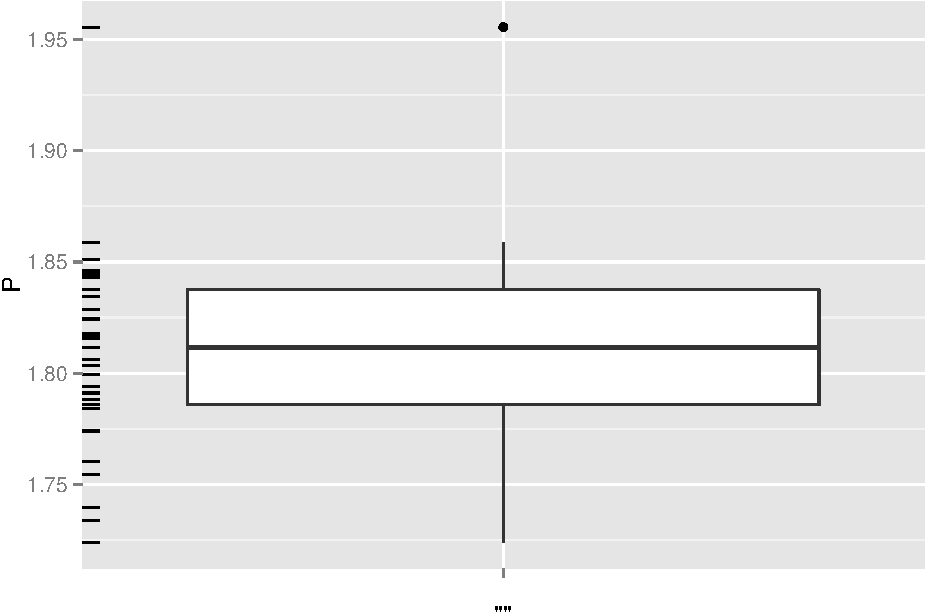
\includegraphics{AnalysisProcedure_files/figure-latex/work_mean_power-1.pdf}

\end{document}
